\begin{figure}[t]\centering
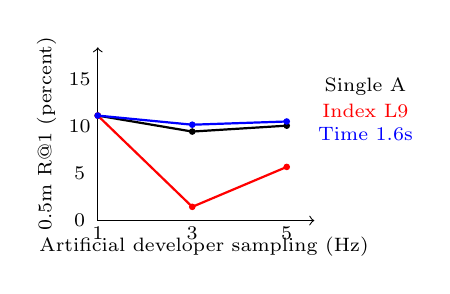
\begin{tikzpicture}[x=1cm,y=1cm]
\draw[->] (0.8,0.35)--(3.55,0.35);\draw[->] (0.8,0.35)--(0.8,2.55);
\node[font=\scriptsize,rotate=90] at (0.15,1.45){0.5m R@1 (percent)};
\node[font=\scriptsize] at (2.15,0.02){Artificial developer sampling (Hz)};
\foreach \x/\label in {0.8/1,2.0/3,3.2/5}{\node[font=\scriptsize] at (\x,0.19){\label};}
\foreach \y/\label in {0.35/0,0.95/5,1.55/10,2.15/15}{\node[font=\scriptsize] at (0.57,\y){\label};}
\draw[black,thick] (0.800,1.683) -- (2.000,1.480) -- (3.200,1.555);
\fill[black] (0.800,1.683) circle (1.2pt);
\fill[black] (2.000,1.480) circle (1.2pt);
\fill[black] (3.200,1.555) circle (1.2pt);
\draw[red,thick] (0.800,1.683) -- (2.000,0.524) -- (3.200,1.031);
\fill[red] (0.800,1.683) circle (1.2pt);
\fill[red] (2.000,0.524) circle (1.2pt);
\fill[red] (3.200,1.031) circle (1.2pt);
\draw[blue,thick] (0.800,1.683) -- (2.000,1.567) -- (3.200,1.608);
\fill[blue] (0.800,1.683) circle (1.2pt);
\fill[blue] (2.000,1.567) circle (1.2pt);
\fill[blue] (3.200,1.608) circle (1.2pt);
\node[font=\scriptsize,text=black] at (4.2,2.05){Single A};
\node[font=\scriptsize,text=red] at (4.2,1.75){Index L9};
\node[font=\scriptsize,text=blue] at (4.2,1.45){Time 1.6s};
\end{tikzpicture}
\caption{Pioneer artificial sampling changes both history duration and gallery coverage. Fixed physical-time alignment is a baseline, not evidence of endpoint-refinement improvement or a new independent collection.}\label{fig:sampling}\end{figure}
